\documentclass[12pt]{article}
\usepackage[utf8]{inputenc}

\usepackage{mystyle}
\usepackage{parskip}
\usepackage{float}
\usepackage[normalem]{ulem}

% Comic Sans
% \usepackage{sansmathfonts}
% \usepackage{fontspec}
% \setmainfont{Comic Sans MS}

% \usepackage{fontspec}
% \setmainfont{Wingdings-Regular.ttf}

% \usepackage{libertine}

% fancy header
\usepackage{fancyhdr}
\pagestyle{fancy}
\rhead{Joseph Sullivan}

\title{Betti Beware---Syzygies Ahead!}
\author{Joseph Sullivan}
\date{October 2024}


\begin{document}

\maketitle

\section{Hartshorne Review}

On projective space $\P^n$, with $S=\C[x_0,\dots,x_n]$, we have the functors
\[
\begin{array}{ccc}
    \QCoh(\P^n) & & \text{graded $S$-modules}\\
     \cF & \qquad\mapsto\qquad & \Gamma_*(\cF) \defeq \bigoplus_{m\in \Z} \Gamma(\cF(m))\\
     \tilde{E} & \mapsfrom & E
\end{array}
\]
satisfying $\tilde{\Gamma_*(\cF)} \cong \cF$. The functor $\tilde{(-)}$ is exact, but $\Gamma_*$ is only left exact.

To restrict to $\Coh(\P^n)$ and finitely generated graded $S$-mod, we (sometimes) need to truncate $\Gamma_*$, so redefine
\[\Gamma_*(\cF) \defeq \bigoplus_{m\geq m_0} \Gamma(\cF(m))\]
for $m_0$ very small.

From now on, 
\begin{itemize}
    \item $\cF\in \Coh(\P^n)$
    \item $E_\cF = \Gamma_* \cF$, a finitely generated module graded $S$-module
\end{itemize}

\section{Betti Numbers and Examples}

\begin{thmdef}
    Let $E$ be a finitely generated graded $S$-module. Then, $E$ has a unique \textbf{minimal graded free resolution} over $S$, i.e., an exact sequence
    \[\cdots \xrightarrow{d_2} P_1 \xrightarrow{d_1} P_0 \to E \to 0\]
    where
    \begin{itemize}
        \item free means $P_i = \bigoplus S(-j)^{b_{i,j}}$ (with finite support)
        \item minimal means $\im d_i \subseteq \fm P_{i-1}$
    \end{itemize}
    We call $P_i$ the \textbf{$i$th syzygy module}.
\end{thmdef}

\begin{proof}
    Graded Nakayama's lemma.
\end{proof}

\begin{rmk}
    In very specific examples---e.g., $\cF=\cI_X$, where you are given generators of the homogeneous ideal $I_X$---you can compute minimal graded free resolutions using Macaulay 2 (or by hand).

    We want to say something about Betti numbers (or even calculate them) for wide classes of coherent sheaves, not just a one off example. Our best friend Koszul complexes will save us.
\end{rmk}

\begin{thmdef}
    Suppose $f_1,\dots,f_r \in S$ is a regular sequence (so $V(f_1,\dots,f_r)$ is a complete intersection/each $f_i$ drops the dimension). Then,
    \[(0 \to S(-\deg f_1) \xrightarrow{\cdot f_1} S \to 0) \otimes \cdots \otimes (0\to S(-\deg f_r) \xrightarrow{\cdot f_r} S \to 0)\]
    is exact, except at degree 0, where the homology is $S/(f_1,\dots,f_r)$
\end{thmdef}

\begin{eg}[Linear subspaces]
    A linear subspace $L\subseteq \P^n$ is a CI of hyperplanes $H_1,\dots,H_r$, so
    \[
        (0 \to S(-1) \xrightarrow{\cdot H_1} S \to 0) \otimes \cdots \otimes (0\to S(-1) \xrightarrow{\cdot H_r} S \to 0),
    \]
    i.e.,
    \[0\to S(-r)^{\binom{r}{r}} \to S(-n+1)^{\binom{r}{r-1}} \to \cdots \to S(-1)^{\binom{r}{1}} \to S^{\binom{r}{0}} \to 0\]
    is exact after tacking on $S/(H_1,\dots,H_r)$, or alternatively replacing $S$ with $(H_1,\dots,H_r)$.
\end{eg}

\begin{eg}[Points in $\P^2$]
    \begin{itemize}
        \item 1 pt is a linear subspace, so get
        \[0 \to S(-2) \to S(-1)^2 \to I \to 0.\]
        \item 2 pts is the CI of a quadric and line, so get
        \[0 \to S(-3) \to S(-2) \oplus S(-1) \to I \to 0.\]
        \item 3 pts has multiple cases:
        \begin{itemize}
            \item Collinear, so CI of a cubic and line, so get
            \[0 \to S(-4) \to S(-3) \oplus S(-1) \to I \to 0.\]
            \item Noncollinear, so general (linear) position.
            
                \textbf{Fact:} $\reg(\cI)=2$, which implies the 0th syzygy module is generated in degrees $\leq2$, and 1st syzygy module in degrees $\leq 3$.

            So, $I$ is generated in degrees $\leq 2$. No line passes through 3 noncollinear points, so $I_1=0$.
            \begin{center}
                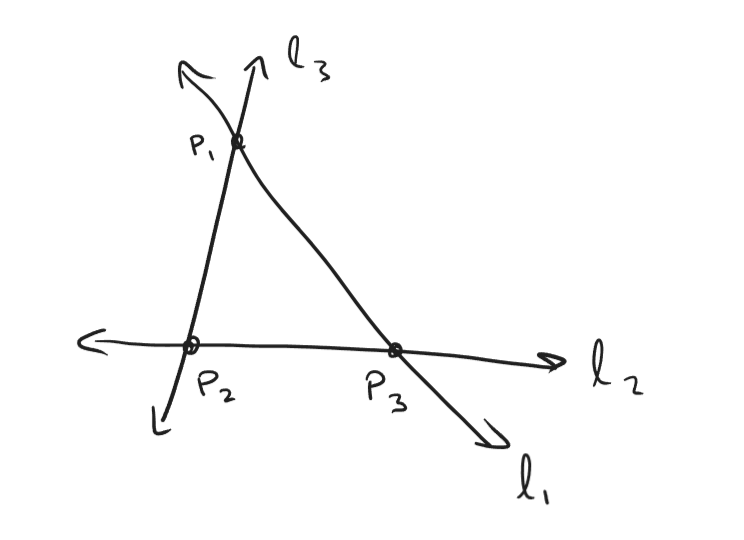
\includegraphics[scale=0.25]{syzygy.png}
            \end{center}
            On the other hand, call $\ell_1,\ell_2,\ell_3$ the lines going through 2 points, so then each $\ell_i \ell_j$ vanish on all points. Furthermore, these form a basis for $I_2$---this is because there is a $\P^5$ worth of conics, and 3 points in general position impose independent linear conditions, giving us a $\P^2$, which is spanned by three points.

            So far, our resolution looks like
            \[S(-2)^3 \to I \to 0.\]
            For the 1st syzygy module, our fact tells us that it is generated in degree 3, so it consists of linear relations on the quadrics. We can do the linear algebra and compute that generators for the linear relations are
            \begin{align*}
                \ell_3 (\ell_1 \ell_2) - \ell_2 (\ell_1 \ell_3) &= 0\\
                \ell_3 (\ell_1 \ell_2) - \ell_1 (\ell_2 \ell_3) &= 0,
            \end{align*}
            so we get
            \[0\to S(-3)^2 \to S(-2)^3 \to I \to 0,\]
            and it ends here (one can check the map is injective, or see that Hilbert's syzygy theorem implies it ends).
        \end{itemize}
    \end{itemize}

    Already we see that this gets complicated as you add in more points, and have to consider all the different special configurations.
\end{eg}

\begin{defn}[Betti Table]
    Usually, we organize the data of the betti numbers into a table, which we index slightly strangely to make it more compact.
    \begin{center}
    \begin{tabular}{c|c c c}
                 & $\cdots$      & $i$      & $i+1$ \\\hline
        $\cdots$ & $\cdots$ & $\cdots$      & $\cdots$ \\
        $j$      & $\cdots$ & $b_{i,i+j}$   & $b_{i+1,i+j+1}$\\
        $j+1$    & $\cdots$ & $b_{i,i+j+1}$ & $b_{i+1,i+j+2}$
    \end{tabular}
    \end{center}
\end{defn}

\section{Regularity}

\begin{defn}
    For $m\in \Z$, $\cF$ is \textbf{$m$-regular} if
    \[H^i(\P,\cF(m-i))=0 \qquad \text{for $i>0$}.\]
    The \textbf{(Castelnuovo Mumford) regularity} $\reg(\cF)$ of $\cF$ is the smallest such $m$.
\end{defn}

\begin{rmk}
    Smaller regularity is ``better'', gives earlier vanishing.
\end{rmk}

\begin{eg}
    $\reg(\cO_{\P^n}(a))=-a$, since all higher cohomology vanishes except potentially the top cohomology, and
    \[H^n(\cO(a+m-n)) = H^0(\cO(-n-1-(a+m-n)),\]
    so to get vanishing we want
    \begin{align*}
        -1-a-m &< 0\\
        m &\geq -a.
    \end{align*}
\end{eg}

\begin{eg}\label{reg-in-SES}
    If $0\to \cF' \to \cF \to \cF'' \to 0$ is exact, then we can often relate their regularities.
    \begin{itemize}
        \item ($\cF',\cF''$ $m$-regular) implies $\cF$ $m$-regular.
        \item ($\cF'$ $(m+1)$-regular and $\cF$ $m$-regular) implies $\cF''$ $m$-regular.
        \item ($\cF$ $m$-regular and $\cF'$ $(m-1)$-regular AND $H^0(\cF(m-1)) \twoheadrightarrow H^0(\cF''(m-1))$) implies $\cF'$ is $m$-regular
    \end{itemize}
    \begin{proof}
        Twist by $\cO(m-i)$, then LES of cohomology
    \end{proof}
\end{eg}

\begin{eg}
    The ideal sheaf $\cI_X$ of $X=\{\text{3 points}\}$ in $\P^2$ in general position has $\reg(\cI_X)=2$. To see this, we compute
    \[H^1(\cI_X(m-1), H^2(\cI_X(m-2)),\]
    and all others vanish by Grothendieck vanishing. To compute these remaining groups, we look at the ideal sheaf sequence
    \[0\to \cI_X \to \cO_{\P^2} \to \cO_X \to 0,\]
    twist it appropriately, and apply sheaf cohomology.

    For $H^1$, we have
    \[H^0(\cO_{\P^2}(m-1)) \xrightarrow{H^0(\text{rest.})} H^0(\cO_{X}(m-1)) \to H^1(\cI_X(m-1)) \to H^1(\cO_X(m-1)),\]
    and $H^1(\cO_X(m-1))=0$, so $H^1(\cI_X(m-1))$ 0 if $H^0$ of restriction is surjective.

    A section of $\cO_X(m-1) = \bigoplus_{i=1}^3 \cO_{P_i}$ is just 3 complex numbers, values assigned to each point, with a generating set for this vector space being $(1,0,0),(0,1,0),(0,0,1)$.
    
    So, we want to know if there exist global sections of $\cO_X(m-1)$ which vanish at 2 points but not the 3rd. This will follow from general position---the condition for vanishing at 2 points will cut down the space of $(m-1)$-forms by 2 exactly dimensions (no fewer), and vanishing on the 3rd will cut down again one more dimension. Though, for this to work out, we need there at least $3$ dimensions worth of $(m-1)$-forms, so we need
    \begin{align*}
        \binom{m-1+2}{2} \geq 3\\
        (m+1)m \geq 6,
    \end{align*}
    which starts at $m=2$. So, for $m\geq 2$, we get $H^1(\cI_X(m-1))=0$.

    For $H^2$, things are much easier. We have the exact sequence
    \[H^1(\cO_X(m-2)) \to H^2(\cI_X(m-2)) \to H^2(\cO_X(m-2)) = H^0(\cO_X(-3-m+2))^\vee,\]
    where the left term always vanishes, and the right vanishes for $m\geq -1$.

    So, indeed, $\reg(\cI_X)=2$.
\end{eg}

\begin{thm}[Mumford]
    Assume $\cF$ is $m$-regular. Then,
    \begin{enumerate}[(i)]
        \item $\cF(m)$ is globally generated
        \item $\Gamma_* \cF$ is generated in degrees $\leq m$.
        \item $\cF$ is $(m+1)$-regular.
    \end{enumerate}
\end{thm}

\begin{proof}[Proof Sketch.]
    The crux is (ii) and (iii), which both follow types of arguments in example \ref{reg-in-SES} applied to the exact sequence which is $\cF$ tensored by the ``sheaf sequence associated to the Koszul complex resolution of $S/\fm$'', which we will see later.

    cohomology vanishing from LESs of sheaf cohomology gets (iii)

    (ii) is equivalent to $V\otimes H^0(\cF(m)) \twoheadrightarrow H^0(\cF(m+1))$, where $V= H^0(\cO(1))$.
\end{proof}

\begin{thm}
    Let $\cF\in \Coh(\P^n)$ with no associated primes of dim 0. Then, $\reg(\cF)=m$ if and only if
    \[b_{i,j}(E_\cF) \leq m+i\]
\end{thm}

\begin{proof}
    If $\reg(\cF)=m$, then $E_\cF$ is generated in degrees $\leq m$, so we can build $P_0$ in free resolution with good Betti numbers. Then, we can control regularity of the kernel (make it $(m+1)$-regular), and continue inductively.

    Conversely, if we have the bound on betti numbers, we can sheafify and use an argument like example \ref{reg-in-SES} to control regularity.
\end{proof}

So, we actually do get our computation for the 3 points in $\P^2$.

\section{Koszul Cohomology}

We can realize Betti numbers as a cohomology theory of sorts, in the following way:

Given a minimal free resolution of $E$
\[0 \to P_k \to \cdots \to P_1 \to P_0 \to 0,\]
(so $\coker d_1 = E$), it is in particular a projective resolution. So, if we tensor with $S/\fm$, its homology computes $\Tor$. Since the resolution is minimal, $\im d_i \subseteq \fm P_{i-1}$, so after tensoring all maps are 0. So,
\[\Tor_i(E,S/\fm) = \bigoplus \C(-j)^{b_{i,j}},\]
or
\[\dim_\C \Tor_i(E,S/\fm)_j = b_{i,j}.\]

But, we can also compute this $\Tor$ the other way, by resolving $S/\fm$ and then tensoring with $E$. The ideal $\fm=(x_0,\dots,x_n)$ is cut out by a regular sequence, so we have the Koszul complex as our resolution,
\[0\to\bigwedge^n V \otimes S(-n) \to \cdots \to \bigwedge^1 V \otimes S(-1) \to \bigwedge^0 V \otimes S \to 0\]
(so cokernel is $S/\fm$, and $V=\C^{n+1}$). Then, we tensor by $E$ and take homology. Taking the $(p+q)$th graded component and looking at the $p$th degree (so matching the Betti table convention), we get
\[\cdots \to \bigwedge^{p+1} V \otimes E_{q-1} \xrightarrow{\delta_{p+1,q-1}} \bigwedge^p V \otimes E_q \xrightarrow{\delta_{p,q}} \bigwedge^{p-1} V \otimes E_{q+1} \to \cdots,\]
and now, indexed by $q$, it is a cochain complex.

\begin{defn}
    We denote the cohomology of this complex by
    \[K_{p,q}(E) := \frac{\ker \delta_{p,q}}{\im \delta_{p+1,q-1}},\]
    called the $(p,q)$th \textbf{Koszul cohomology} group of $E$, but of course this is just a way to compute $\Tor_p(E,S/\fm)_{p+q}$.
\end{defn}

Along the way, we've proved Hilbert's syzygy theorem, that there are no syzygies in degrees beyond $n$, so that says something about Betti numbers. The advantage to describing Betti numbers as a sort of cohomology theory is that we'll also get a Serre duality statement.

\section{Canonical Curves}

Now this is the section where I speak at you and prove nothing. If $C$ is a smooth projective curve of genus $g\geq 2$ and non-hyperelliptic (i.e., non 2-gonal), then the complete linear series of $\omega_C$ gives an embedding
\[i: C \hookrightarrow \P^{g-1}\]
since Riemann-Roch gives
\begin{align*}
    h^0(\cO_C) - h^1(\cO_C) &= \deg(\cO_C) - g + 1\\
    h^0(\cO_C) - h^0(\omega_C) &= \deg(\cO_C) - g + 1\\
    1 - h^0(\omega_C) &= 0 - g + 1\\
    h^0(\omega_C) &= g,
\end{align*}
and one can show $\omega_C$ globally generated/very ample by computing $h^0(\omega_C-P)$ and $h^0(\omega_C-P-Q)$.

\textbf{Question.} What can we say about the Betti table of $C\hookrightarrow \P^{g-1}$, i.e., what does the resolution of $\Gamma_* \cO_C$ look like?

Let's apply our machinery from before. First, we'll prove that $\cO_C$ is $3$-regular (as a sheaf on $\P^{g-1}$), but since it is the pushforward of a sheaf on a curve, we only have to worry about the vanishing of an $H^1$. So, we study
\[H^1(\cO_C(m-1)) = H^1(\omega_C^{\otimes(m-1)}) \cong H^0(\omega_C^{\otimes (2-m)})^\vee,\]
which vanishes whenever $2-m<0$, so $m>2$, so $m\geq 3$. So, our Betti table is all 0s after row 3.

Then, there's a way to compute Koszul cohomology as sheaf cohomology of ``kernel bundles'' on $C$, where we can apply Serre duality to eventually compute
\[K_{p,1} = K_{g-2-p,2},\]
so we get a symmetry in our table.

Also, resolutions end in after $g-2$, since $C$ is projectively Cohen Macaulay (due to some cohomology vanishing), so we can apply Auslander-Buchsbaum to compute the length of minimal resolutions.


Some classical theorems about canonical curves.
\begin{thm}
    \begin{enumerate}[(i)]
        \item (Noether) $C$ is projectively normal/$\omega_C$ is normally generated
        \item (Petri) The homogeneous ideal $\cI_{C/\P^{g-1}}$ fails to be generated by quadrics iff trigonal or smooth plane quintic.
    \end{enumerate}
\end{thm}

We will reframe this result, and come up with an extension called \textbf{Green's conjecture}.
\begin{enumerate}[(i)]
    \item Noether's result states that for $C$ genus $g\geq 2$ and NOT hyperelliptic, we have projective normality, i.e., we have the surjections
    \[H^0(\cO_{\P^{g-1}}(k)) \twoheadrightarrow H^0(\cO_C(k)).\]
    So, when building a resolution of $\Gamma_* \cO_C$ over $S=\C[x_1,\dots,x_g]$, our first step is just surjecting with $S$, i.e., it will look like
    \[? \to S \to \Gamma_* \cO_C \to 0,\]
    and the kernel of the surjection is exactly $I_C$, so the next step is generating $I_C$.

    \item Petri's result is that, when we continue our resolution, we won't need to use $S(-3)$ or higher in the next step, i.e.,
    \[? \to S(-2)^{b_{1,2}} \to S \to \Gamma_* \cO_C \to 0,\]
    (where we aren't interested in when $I_C$ has any degree $1$ generators, because then $C$ lands in some subspace)
\end{enumerate}

We can reframe this by defining the following property:
\begin{defn}
    $X\hookrightarrow \P^n$ satisfies \textbf{property $(N_k)$} if
    \[K_{p,q}(X) = K_{p,q}(\Gamma_*\cO_X) = 0\]
    for $p\leq k$ and $q\geq k$. In terms of Betti numbers,
    \[b_{i,j} = 0\]
    for $i\leq k$ and $j\geq i+k$, and in terms of Betti tables, (assuming no linear generators of $I_C$)
    \begin{center}
    \begin{tabular}{c|c c c c c}
        $(i+j)\backslash i$ & 0 & 1 & $\cdots$ & $k$ & $k+1$ \\\hline
        0        & 1 & 0        & $\cdots$         & 0         & 0\\
        1        & 0 & $\square$   & $\cdots$  & $\square$    & ?\\
        2        & 0 & 0        & $\cdots$         & 0         & ?\\
        $\vdots$ & 0 & 0        & $\cdots$         & 0         & ?
    \end{tabular}
    \end{center}
\end{defn}

So,
\begin{enumerate}[(i)]
    \item Noether: not hyperelliptic is $N_0$
    \item Petri: not hyperelliptic or trigonal or smooth plane quintic is $N_1$
\end{enumerate}

\textbf{Conjecture.} (Green) The smallest $k$ where property $(N_k)$ fails is 
\[\min\{\deg(A)-2(h^0(A)-1) \mid A\in \Pic(C), h^0(A)\geq 2, h^1(A) \geq 2\}\]
called the Clifford index $\mathrm{Cliff}(C)$.

There are classical theorems which state $C$ is hyperelliptic iff $\mathrm{Cliff}(C)=0$ (so $(N_0)$ fails), and $C$ is trigonal/smooth plane quintic iff $\mathrm{Cliff}(C)=1$ (so $(N_1)$ fails)

It is also known that if $k \leq \mathrm{Cliff}(C)$, then $k\geq \mathrm{Cliff}(C)$ (so definitely captures lots of counterexamples to $(N_k)$), so the crux is to show that ALL counterexamples are captured by $\mathrm{Cliff}(C)$, i.e., if $k<\mathrm{Cliff}(C)$, then $(N_k)$ holds.

Voison proved Green's conjecture for a general curve, in which case $\mathrm{Cliff}(C) = \left[\frac{g-1}{2}\right]$


\nocite{*} % Include all references in refs.bib regardless of whether they are referenced or not
\bibliographystyle{plain} % We choose the "plain" reference style
\bibliography{2024fall/syzygy_refs} % Entries are in the refs.bib file

\end{document}